\documentclass{article}
\usepackage[utf8]{inputenc}

\title{IF699 - Aprendizagem de Máquina}
\author{Marcus Filipe Barbosa de Menezes}
\date{Novembro, 2019}

\usepackage{natbib}
\usepackage{graphicx}

\begin{document}
\maketitle

\section{Introdução}
O Aprendizado de Máquina é um dos temas mais atuais e de rápido crescimento na área da informática, com diversas possibilidades de usos, essa técnica é feita de modo similar ao que os seres humanos aprendem, por meio da experiência e tentativa e erro, recebendo dados reais e melhorando sua performance. Existem três principais tipos de machine learning, o supervisionado, o não supervisionado e o aprendizado por reforço.\cite{3machinelearning}

\begin{figure}[h!]
\centering
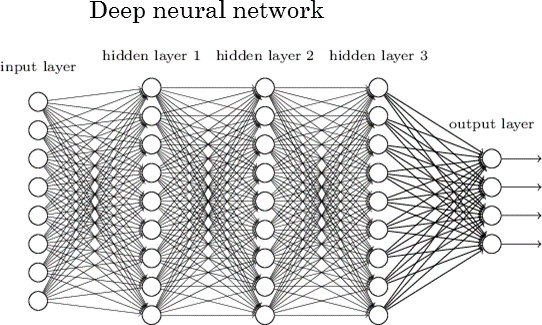
\includegraphics[scale=0.8]{neuralnetwork.png}
\caption{Rede Neural de Aprendizado de Máquina}
\label{fig:Neural Network}
\end{figure}

\section{Relevância}O Aprendizado de Máquina para determinadas tarefas é muito mais rápido e preciso do que o do humano, visto que o computador pode realizar simulações de aprendizado muito mais rápido do que nós, além de conseguir analisar uma grande quantidade de dados ao mesmo tempo. Por isso, a quantidade de aplicações para estas técnicas é enorme e cada ano descobrimos novas aplicações, tais como: análise de dados, reconhecimento de voz, reconhecimento facial, direção de carros autônomos\cite{tesla}, treinamento de robôs \cite{robocin}, aprendizagem de jogos \cite{alphago}.

\section{Relação com outras disciplinas}
A disciplina de Aprendizagem de Máquina possui como requisito o término da disciplina IF685 - Gerenciamento de dados e informação, visto que é um tópico que lida com grandes fluxos de dados e é imprescindível a habilidade de interpretá-los. Além disso, a disciplina possui uma boa interdisciplinaridade com a cadeira IF702- Redes Neurais, dado o grande uso dessas redes similares ao nosso sistema nervoso para a Aprendizagem de Máquina\cite{neural}. 

\bibliographystyle{plain}
\bibliography{mfbm}
\end{document}
